\chapter{The LHC accelerator and the CMS experiment}\label{chapter:lhc-cms}
\section{The Large Hadron Collider}\label{sec:lhc}

The Large Hadron Collider (LHC) at the European Organisation for Nuclear Research (CERN)~\cite{Bruning:782076}, in Geneva, Switzerland is the highest-energy particle accelerator constructed to date. 
It is designed to operate at a centre of mass (CoM) energy of 14\TeV, through two 7\TeV proton beams travelling in 2808 bunches of up to $1.15 \times 10^{11}$ protons at a collision rate of 25\ns which corresponds to a design luminosity of $10^{34}\percms$~\cite{Bayatian:2006zz}. 
The LHC can also operate in a heavy-ion mode, where lead ions are collided at 2.76\TeV per nucleon usually for one month a year.

The beams collide at four interaction points around the LHC, with one of the four major experiments being based at each of them. 
The experiments are: A Toroidal LHC Apparatus (ATLAS)~\cite{Aad:2008zzm} and the Compact Muon Solenoid (CMS)~\cite{oldcms} detectors, which are the two multi-purpose experiments; the Large Hadron Collider beauty (LHCb)~\cite{Alves:2008zz} is an experiment which specialises in b-physics and; A Large Ion Collider Experiment (ALICE)~\cite{Aamodt:2008zz}, which as the name suggests, specialises in heavy ion physics.
Three smaller experiments are situated close to one of the four main experiments and use the same collision points.
Both the TOTal Elastic and diffractive cross section Measurement (TOTEM)~\cite{Anelli:2008zza} and LHC-forward (LHCf)~\cite{Adriani:2008zz} experiments study diffractive physics in the very-forward regions of collisions at the CMS and ATLAS experiments' collision points respectively.
Monopole and Exotics Detector At the LHC (MoEDAL)~\cite{Pinfold:2009oia} shares the LHCb experiment's cavern and performs direct searches for magnetic monopoles and highly ionising stable and pseudo-stable massive particles.

Currently there are three planned phases of operation for the LHC~\ref{fig:lhc-planning}: ``Phase-0'' will see the preparations for 14\TeV operations; ``Phase-I'' will see the accelerator prepared for high luminosity operations; and ``Phase-II'' will see modifications for very high luminosity operations~\cite{ECFA}. Any proposed upgrades of the detectors will naturally have to coincide with the shutdowns of the LHC.

\begin{figure}[htbp]
\begin{center}
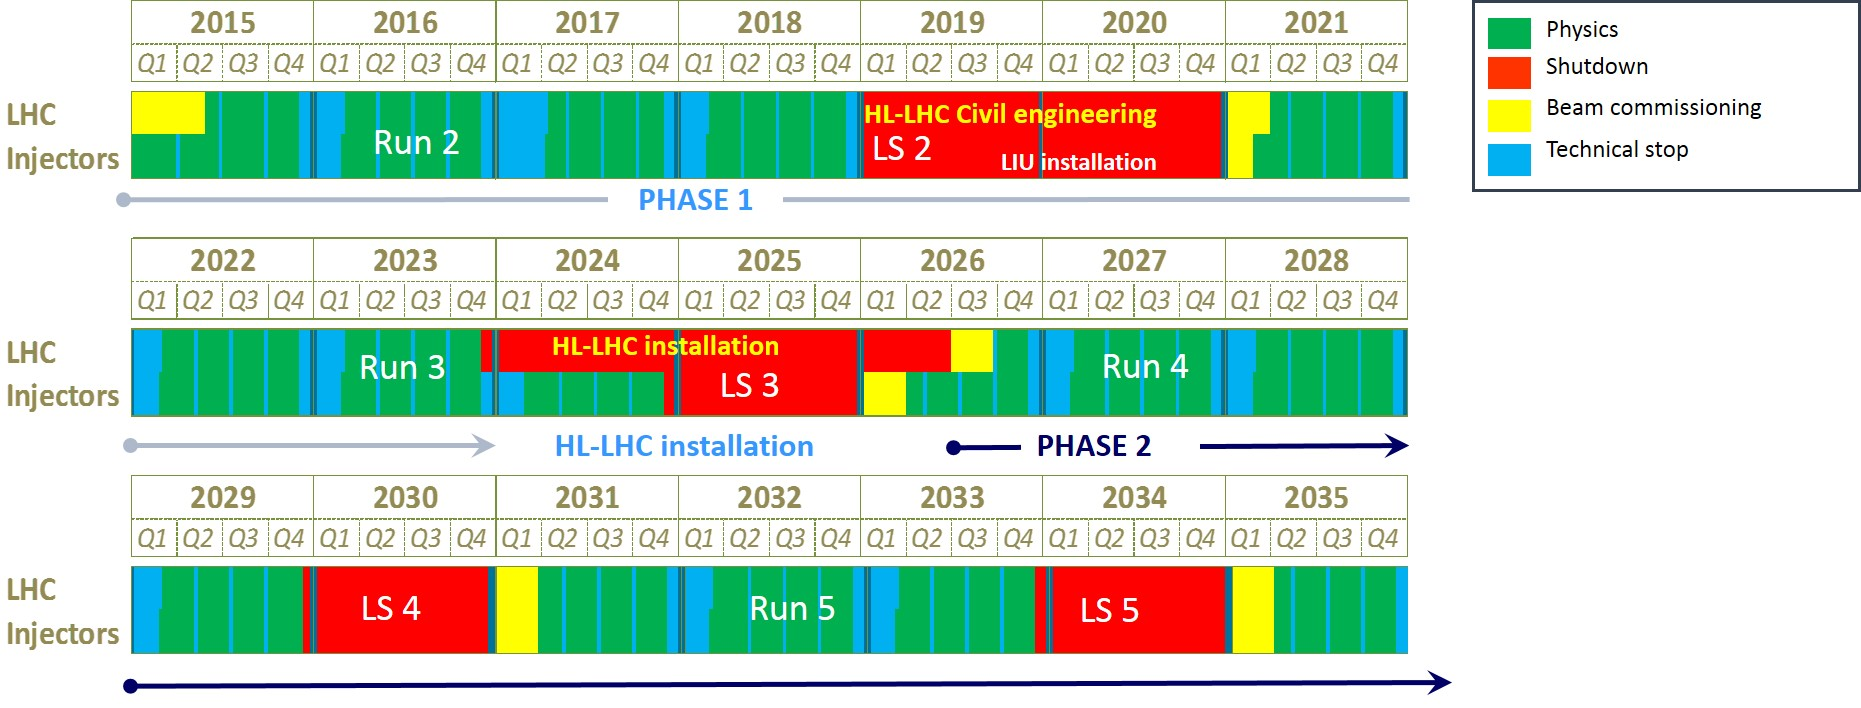
\includegraphics[width=0.97\textwidth]{figs/lhc/LHC-Planning.jpg}
\caption{Overview of the plan for the LHC and its injectors from 2015 to 2035~\cite{P2TrackerTDR}. Data taking for physics is indicated in green, long shutdowns in red, beam commissioning in yellow and technical stops in blue.}
\label{fig:lhc-planning}
\end{center}
\end{figure}

\editComment{Insert LHC timetable schedule image}

\subsection{Accelerator Complex}
When operating in proton-proton mode, the preparation of the LHC beams starts at Linear accelerator 2 (Linac2). 
Protons from a hydrogen gas source are accelerated to 50\MeV and are injected into the Proton Synchrotron Booster which accelerates the protons to 1.4\GeV before injection into the Proton Synchrotron (PS). 
In the PS, the protons are accelerated to 26\GeV and are injected into the Super Proton Synchrotron (SPS) where they are accelerated to 450\GeV before finally entering the LHC~\ref{fig:cern-accelerator-complex}. 
When operating with lead ions, Linear accelerator 3 (Linac3) is used to initially accelerate the ions before injecting them into the Proton Synchrotron Booster, before the ions use the same accelerators as the protons do to prepare them for use in the LHC~\cite{Bruning:782076}. 

Sixteen Radio Frequency (RF) cavities (eight per beam), each operating at frequency of 400\MHz, at a temperature of 4.5K, and delivering a maximum of 2 MV, are used to accelerate the two beams up to their designed operational energies of 7\TeV over the course of circa twenty minutes.
Each of the two beams are accelerated in separate beam pipes, circulating in opposite directions,and requires 1232 dipole magnets to bend them along their circular path and 392 quadrupole magnets to focus them, with each magnet producing a 8.3T field whilst operating at 1.9K.
A more detailed description of the LHC accelerator chain at CERN can be found in~\cite{Schindl:397574}. 

\begin{figure}[htbp]
\begin{center}
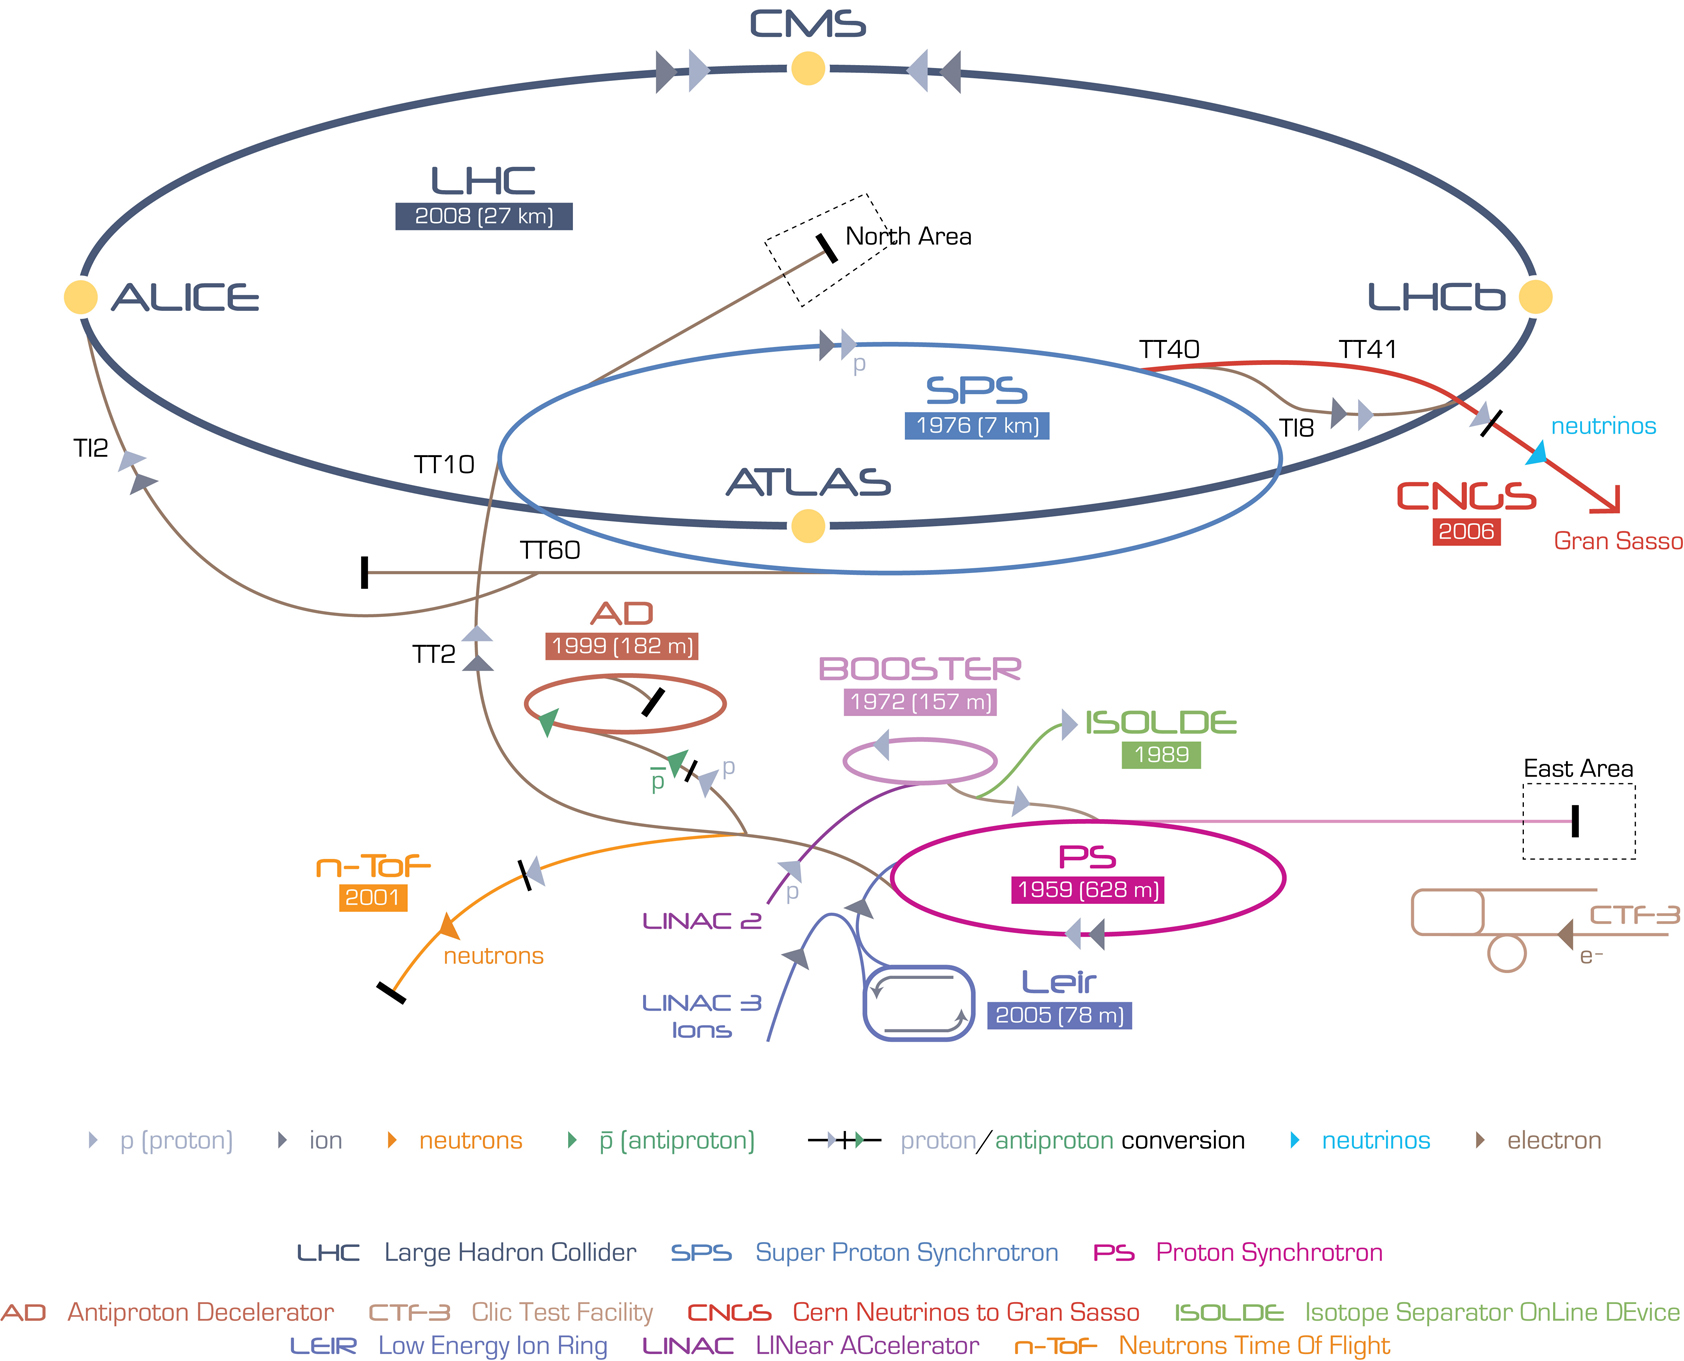
\includegraphics[width=0.97\textwidth]{figs/lhc/Cern-Accelerator-Complex.jpg}
\caption{CERN complex, including the various linear accelerators, synchrotrons, LHC, LHC detectors and other aspects of the complex.}
\label{fig:cern-accelerator-complex}
\end{center}
\end{figure}

\subsection{Motivation}
The core motivations behind the LHC are to shed light on the nature of the electroweak symmetry breaking, which the Higgs was presumed and found to be responsible, and to probe the consistency of the SM above the \TeV level through precision measurements of SM parameters and the Higgs mechanism.
Alternative theories to the SM, such as SUSY theories, additional dimensions or new fundamental forces and particles are expected to emerge at and above the TeV level, giving the potential to ascertain whether these theories have any basis beyond mere conjecture~\cite{Bayatian:2006zz}.

In order to explore and permit the discovery of physics at the \TeV level, the total centre of mass energy has to be greater than the energy region being explored as, due to the composite nature of the proton, only a fraction of the collision centre of mass energy is available.
Access to physics beyond the \TeV level is not excluded	however, as some signals would be ``unmissable'', but the majority of physics would be limited by statistics.
Compared to the total inelastic cross section, the production cross section of the Higgs boson and hypothesised SUSY particles, if they have \TeV masses (and exist), are predicted to be many orders of magnitude smaller (see Fig.~\ref{fig:crossSections}).

\begin{figure}[htbp]
\begin{center}
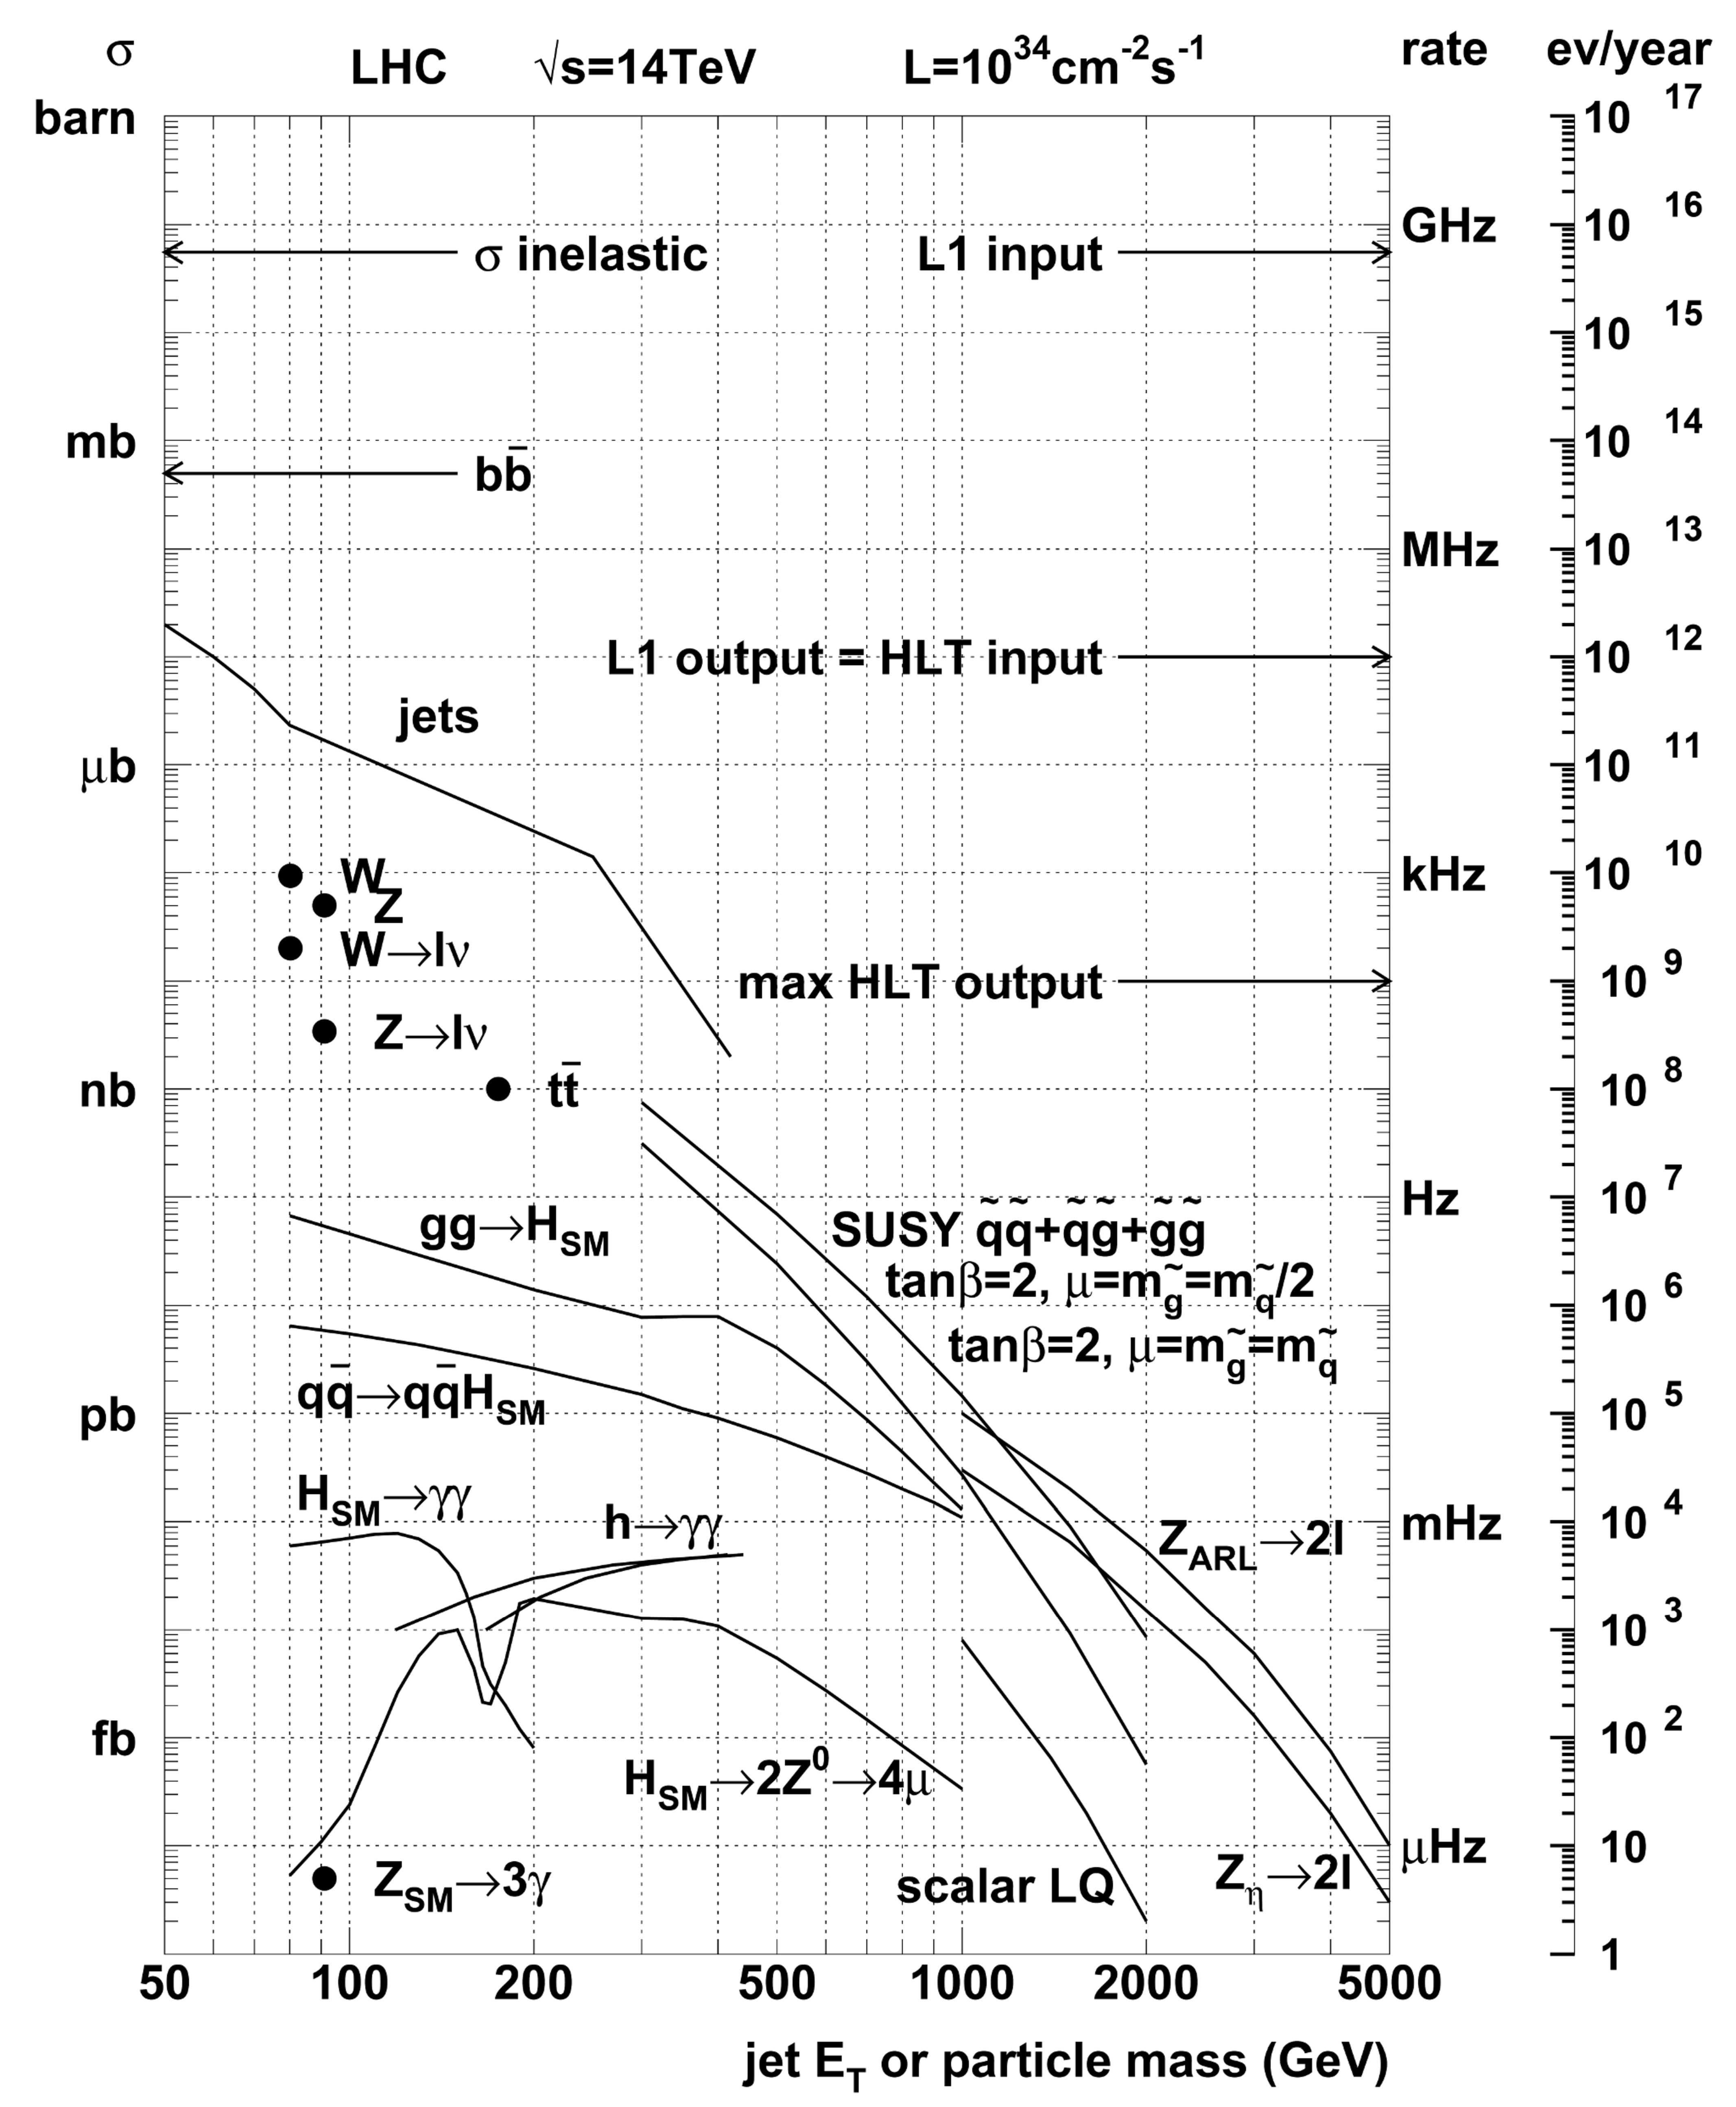
\includegraphics[width=0.55\textwidth]{figs/cms/crossSections.pdf}
\caption{Inclusive proton-proton cross sections for various physics processes, as a function of jet \ET or mass, expected at the LHC at a luminosity of $10^{34}\percms$~\cite{Dasu:2000ge}.}
\label{fig:crossSections}
\end{center}
\end{figure}

Measurements of such processes, as well as precision measurements of SM parameters, require a high interaction rate, and consequently the LHC has a high beam luminosity so that there sufficient statistics available.
Protons are delivered in 2808 bunches per beam, as opposed to a continuous beam, which at design luminosity will separated by 25ns, resulting in an event rate of 40\MHz and an average of 25 inelastic proton-proton interactions, named pile-up (\PU) for each bunch crossing~\cite{Bruning:782076,Ball:2007zza}. 
This high event rate presents the experiments with the data acquisition and readout challenges, whilst retaining excellent signal to background resolution and sufficient radiation hardness in order to withstand the expected fluence.
The primary motivation behind operating the LHC in a heavy-ion mode is to search for evidence of the plasma of quarks and gluons, which is made possible through the resultant production of QCD matter under extreme temperature, density and low momentum fractions of partons~\cite{Baur:687318}.

\section{The Compact Muon Solenoid}\label{sec:cms}
\subsection{Overview}
The Compact Muon Solenoid (CMS)~\cite{oldcms} is a large, general purpose, hermetic particle detector and the smaller of the two multi-purpose experiments operating at the LHC at CERN.
The experiment is divided into a central cylindrical barrel section and two endcap disk sections at each end of the barrel.
A superconducting solenoid encompasses, moving from the interaction point at the centre of the detector outwards, an all silicon tracking detector, a homogeneous lead tungstate ($PbWO_{4}$) electromagnetic calorimeter (ECAL)and hadronic calorimeter (HCAL) comprised of plastic scintillating tiles interspaced with brass absorbers.
Beyond the solenoid there is an outer hadronic calorimeter (HO) and interspaced between the iron return yoke are three different types of Muon Detectors.
There is also a pair of very-forward calorimeters (HF) in the extended rapidity region.

\begin{figure}[htbp]
\begin{center}
\includegraphics[width=0.75\textwidth]{figs/cms/cms_160312_02.pdf}
\caption{Cutaway diagram of CMS’s layers, illustrating its onion-like nature and the location of the detecting technologies within~\cite{Sakuma:2013jqa}.}
\label{fig:cms-cutaway}
\end{center}
\end{figure}

These detectors were designed in order to investigate the wide range of physics phenomena in the LHC's physics program, resulting in the accurate and precise identification and measurement of electrons, photons, jets and muons over both a large energy and momenta range.
Full detector resolution is achieved across $|\eta| < 3.0$, with the hadronic calorimetry having an extended coverage up to $|\eta| < 5.0$ in order to ensure good dijet mass and \MET resolutions.
Sufficient radiation hardness for the expected high fluence and data acquisition and trigger systems required to handle to event rate of the LHC environment had to be considered in the design of the various detectors.

The coordinate system adopted by the CMS experiment has the origin at the nominal interaction point at the centre of the detector. 
The z-axis is parallel to the anti-clockwise proton beam (i.e. towards the Jura mountains from the detector), the x-axis points towards the centre of the LHC, and the y-axis points vertically upwards.
The azimuthal angle, $\phi$, is the angle measured from the x-axis in the x-y plane and the polar angle, $\theta$, is the angle measured from the z-axis.
Pseudorapidity, defined as $\eta \equiv -ln\tan(\theta/2)$, is usually used in lieu of $\theta$ as when the mass considered is negligible $\eta$ converges towards rapidity, defined as $y \equiv	1/2 ln(E+p_{z}/E-p_{Z})$, which is Lorentz invariant along the z-axis.
As such, variables transverse to the z-axis (i.e. the beam line), such as the transverse energy (\ET), momentum (\pT), and missing energy (\MET), depend only on their x and y components.

\subsection{Tracker}\label{subsec:tracker}
The tracker, measuring 5.8m with a 2.5m radius over $|\eta| < 2.5$, surrounds the interaction point, and is designed to provide efficient precision trajectory measurements of charged particles emerging from collisions and precise reconstruction of vertices, whilst operating in a harsh radiation environment (max flux $\approx 10^{7}/s$) and minimising the number charged particles interacting with the tracker (i.e. scattering, producing Bremsstrahlung).
Silicon fulfils these requirements and is used in the inner pixel detector, surrounding the interaction point, and microstrip detector, which encloses the pixel detector.
The high fluence expected closest to the interaction point requires the high granularity pixels provide in order to ensure a low channel occupancy, but the particle flux from $r < 20\cm$ is sufficiently low enough that microstrips can be used without compromising reconstruction efficiency.

\begin{figure}[htbp]
\begin{center}
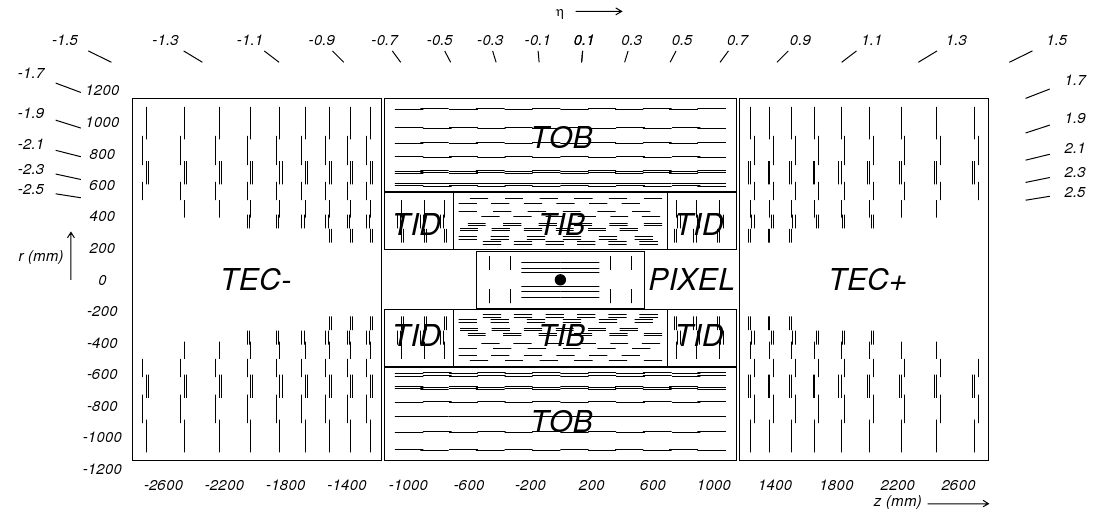
\includegraphics[width=0.97\textwidth]{figs/cms/fig_cmstracker.png}
\caption{Schematic of the CMS tracking detector, displaying the interaction point in the centre and the location the sub-detectors and through the arrangement of the lines, their modules. The double lines present in the microstrip tracker denoting modules with double sided sensors~\cite{Sprenger:2010ss}.}
\label{fig:tracker}
\end{center}
\end{figure}

\subsubsection{Silicon Microstrip Tracker}
The silicon microstrip detector is comprised of four parts: the Tracker Inner Barrel (TIB) and Tracker Inner Disks (TID) from $20 < r < 55\cm$, and the Tracker Outer Barrel (TOB) and Tracker EndCaps (TEC) from $55 < r < 116\cm$.
The sensors are rectangular in the barrel region and trapezoid in the endcaps and all consist of singled sided strips of p+-type implants on n-type silicon which are connected to readout chips (ROCs) by aluminium strips.
A total of 9.3 million sensors are used across all four parts, covering an area of 198 $\unit{m}^{2}$.

The TIB provides coverage up to $|z| = 65\cm$ and is comprised of four layers, with the strips having a pitch of 80\mum for the inner two layers and 120\mum for the outer two layers, and a thickness of 320\mum and a typical length of 10\cm across all four layers.
Three disks on each side of the TIB form the TID. 
Each disk is formed of three rings and the sensor pitches across the rings vary between 81-158\mum, but have a thickness of 320\mum throughout.
Surrounding the TIB and TID is the TOB,	which is comprised of six layers which provide coverage up to $|z| = 110\cm$.
In the outer microstrip tracker, increased strip thickness, length and pitch are used in the where the radiation levels are lower so that a similar occupancy and signal to noise ratio to the inner microstrip tracker can be maintained.
The pitch of the strips vary from 183\mum for the inner four layers to 122\mum for the outer two layers, with all having a thickness of 500\mum and a typical length of 25\cm. 
The TEC's nine disks per endcap extend coverage from $|z| = 120\cm$ to $|z| = 280\cm$, with the number of rings per disk varing from four to seven depending on the disk's position in z.
The thickness of the sensors in the TEC are 320\mum and 500\mum in the three innermost rings and the rest respectively.
A number of ``stereo'' modules of two back to back sensors are used in the inner two layers of the TIB and TOB, the inner two rings of the TID and the inner two and the fifth rings of the TEC.
These sensors are aligned at an angle of 100 mrad to each other, allowing measurements of both the $r-\phi$ and r-z coordinates, to a point resolution of 23-34\mum $r-\phi$ and 23\mum in z and 35–52\mum r-phi and 52\mum in z in the TIB and TOB respectively.

\editComment{WRITE BIT ABOUT TRACK RECO EFF AND RESOLUTIONS FOR 2016}

\subsubsection{Silicon Pixel Tracker}
The original ``Phase-0'' silicon pixel detector was comprised of three 53.3\cm long barrel layers at mean radii of 4.4, 7.3 and 10.2\cm and two endcap disks either side of the barrel at $|z| = 34.5$ and 46.5\cm that extend from $r = 6.0$ to 15\cm.
The pixel sensors consist of n+-type implants  on n-type silicon which are connected by indium bump-bonds to highly integrated ROCs.
Each of the 66 million pixels measures $100 \times 150\mum^{2}$, covering a total surface area of 1.06 m$^{2}$, with point resolutions of 10\mum in $r-\phi$ and 20\mum in z, which provides the granularity required to have a high track reconstruction efficiency and to be able to precisely calculate the track impact parameters and vertex position.

The original pixel detector was designed to operate a nominal instantaneous luminosity of $1 \times 10^{34}\percms$, however, with the ``Phase-I'' LHC conditions of increased \PU from running at a higher instantaneous luminosity with the same 25\ns bunch spacing, the detector will suffer track reconstruction efficiency degradation due to radiation damage.
Therefore during the End of Year Technical Stop that took place between data taking in 2016 and 2017, the pixel detector was completely replaced.
A more detailed description of the Phase-I Pixel detector can be found in~\cite{CMS:2012sda}, given that none of the results discussed in~\ref{sec:results} involve data collected after 2016.
%%Like the original pixel detector, the Phase-I detector's 124 million pixels also measure $100 \times 150\mum^{2}$ (covering a total surface area of 1.95 $m^{2}$) and the sensors are also n+-type implants on n-type silicon.
%%The Phase-I Pixel detector is comprised of four 54.9\cm long barrel layers at mean radii of 3.0, 6.8, 10.9 and 16.0\cm and three endcap disks at each end of the barrel at $|z| = 29.1, 39.6 and 51.6\cm$ that extend from $r = 4.5 to 16.1\cm$.

\editComment{WRITE BIT ABOUT TRACK RECO EFF AND MAYBE RESOLUTIONS FOR 2016 TOO?}

\subsection{Electromagnetic Calorimeter}\label{subsec:ECAL}
Beyond the tracker, the ECAL~\cite{CMS:1997ysd,CMS:2002xia}, a homogeneous calorimeter, measures the energies of electrons and photons using lead tungstate scintillating crystals. 
The choice of using lead tungstate crystals was based on the needs of both having a compact detector which could fit with the HCAL inside the solenoid and containing the showers' energy within this calorimeter, which were met with its short radiation length (0.89\cm) and small Molier\'{e} radius (2.2\cm).

61,200 crystals are mounted in the barrel, with 7,324 crystals for each endcap.
As the crystals only emit a small amount of scintillation light, the photodetectors used to amplify the light must be able to operate within the solenoid's field and and withstand the high radiation environment.
Avalanche photosdiodes and the more radiation hard vacuum photodiodes are used in the barrel and endcap regions respectively.
The emitted light emitted by these crystals is short, well defined and fast, with 80\% collected within one 25\ns bunch crossing, with the signals being digitised on-detector and buffered until a Level-1 Trigger decision has been made.

The barrel and endcap cystal systems are supplemented by a Preshower (ES)~\cite{Loos:539819} device, located in front of the ECAL endcaps, for discrimination between neutral pions and photons within the fidicial region $1.653 < |\eta| < 2.6$.
For each detector, two lead radiators initiate the electromagnetic showers and two silicon strip sensors, orthogonal to one another to provide fine resolution, are placed after the radiators measure the energy deposited.
The thickness of the radiators was chosen to ensure ~95\% of incident photons shower before reaching the second silicon strip sensor, namely two and one radiation lengths for the first and second lead radiators respectively.

\begin{figure}[htbp]
\begin{center}
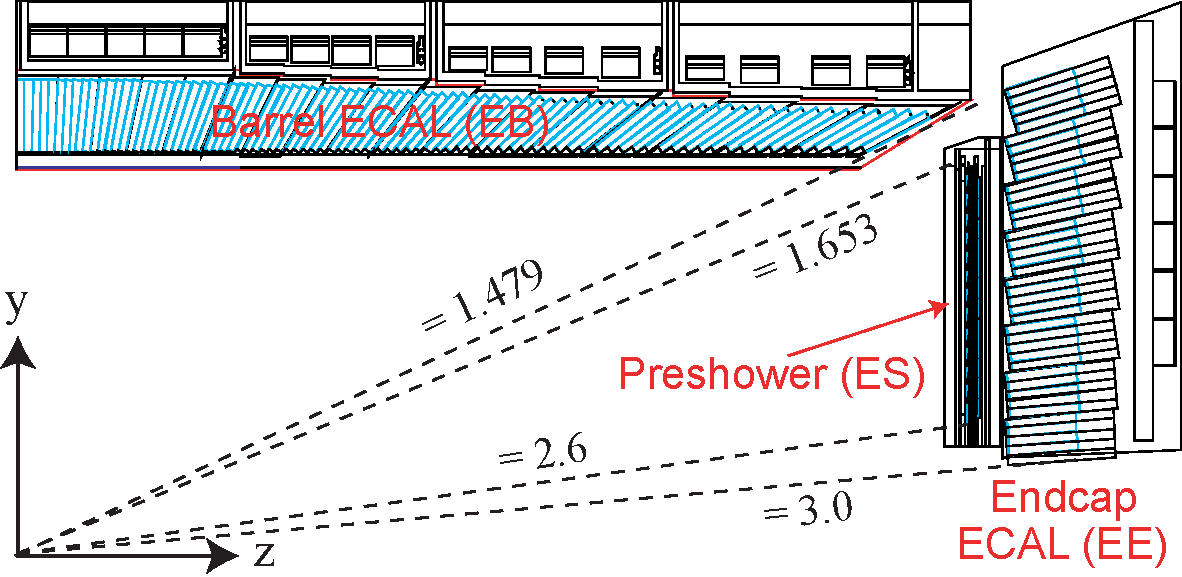
\includegraphics[width=0.97\textwidth]{figs/cms/ECAL_Transverse_section.pdf}
\caption{Layout of one quadrant of the ECAL system, illustrating locations of the various subsystems~\cite{Bayatian:2006nff}.}
\label{fig:ecal}
\end{center}
\end{figure}

\editComment{WRITE BIT ABOUT ENERGY RESOLUTION FOR 2016}

%Following the excellent performance during Run I of the LHC, with an energy resolution of 0.3\% exceeding the design value of 0.5\%, the ECAL has continued to perform admirably, with .... \cite{TeixeiradeLima:2017tmj} %%ECAL performance Run II

\subsection{Hadronic Calorimeter}\label{subsec:HCAL}
Hadronic particles penetrate through the ECAL into the HCAL~\cite{CMS:1997xji}, where hadronic jets have their energies measured and are contained for determination of the missing transverse energy and protection of the muon detectors~\cite{HCAL:tdr}.
As such, the HCAL was designed to have as much absorber material within the solenoid coil as practical. 
The barrel (HB) and and endcap (HE) both use plastic scintillator tiles interspersed between brass and steel absorber plates, with the latter being used for the external plates for structural strengthening.
Wavelength shifting fibres embedding in the tiles converts the scintillated light and channels it to hybrid photodiodes.
The HB covers the rapidity range $|\eta| < 1.4$, with the HE overlapping it and providing coverage over the range $1.3 < |\eta| < 3.0$.

Due to space constraints within the solenoid, the HB cannot fully contain hadronic showers and as such is supplemented by an additional calorimeter in the barrel region outside the coil (HO). Given the outer hadronic calorimeter's limited size and function, it will not be discussed further here, but a thorough description of the HO can be found in~\cite{HO}.

The forward calorimeters (HF)~\cite{HF} overlap with the HE and cover the $2.9 < \eta < 5.0$ rapidity region.
As the forward region experiences the most severe radiation environment, the technology used must be able to withstand such large radiation doses~($10^{9}$ rad). 
Interspaced between steel absorbers, quartz fibres are used produce Cherenkov light due to their radiation hardness, fast response time, production of Cherenkov radiation above a certain energy threshold (thus ignoring low energy particles), and ability to give directional information due to the light being strongly correlated with the showers' trajectories.
The Cherenkov light produced is transmitted down the fibres to individually shielded photomultiplier tubes contained in readout boxes.

\editComment{WRITE BIT ABOUT ENERGY RESOLUTION FOR 2016}

\subsection{The Superconducting Solenoid}\label{subsec:magnet}
One of the defining features of the CMS detector is the superconducting solenoid which encompasses the silicon tracker and calorimetry~\cite{Acquistapace:1997fm,Herve:2000}.
The 220T cylindrical coil measures 13m long, has a 5.9m inner diameter, is situated inside a vacuum tank where it is cooled to its operation temperature by liquid helium to 4.5K, and operates at magnetic field of 3.8 Tesla\footnote{Whilst the solenoid was designed to operate at 4T, the CMS collaboration chose to operate it at 3.8T in order maximise the lifetime of the apparatus}.
The large bending power within the solenoid not only provides excellent momentum resolution for charged particles within the tracking detector, but it also prevents low transverse momentum charged particles from reaching the calorimetry and negatively impacting on energy resolution and isolation efficiency.
An iron return yoke guides and contains the return magnet field, which is sufficiently strong ($\approx$ 1.7T in the barrel and outermost endcap disk) enough to enable accurate momentum resolution for tracking and charge identification of high momentum ($\approx$ 1\TeVc) muons.

\begin{figure}[htbp]
\begin{center}
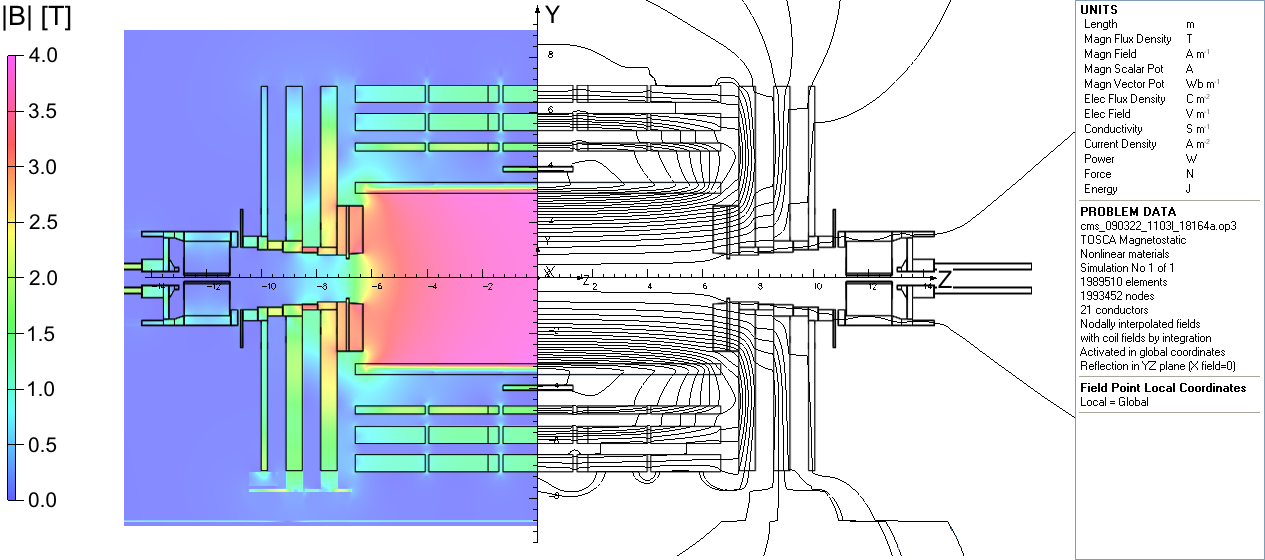
\includegraphics[width=0.97\textwidth]{figs/cms/cms_magnetic_field.png}
\caption{Longitudinal section of the CMS detector, illustrating the predicted magnetic field strength (left) and field lines (right) for the operational central magnetic flux density of 3.8T~\cite{Chatrchyan:2009si}.}
\label{fig:magneticField}
\end{center}
\end{figure}

\subsection{Muon Detectors}\label{subsec:muon chambers}
Detecting muons is incredibly important for CMS (as implied by the experiment’s name), given many of the signatures of interesting events involve them, including those from SUSY models and the so called “gold-plated” SM Higgs decay into a pair of $Z^{0}$ bosons, which in turn decay into four muons. 
Being Minimum Ionising Particles (MIPs), muons pass through the detector and past the magnet with minimal interaction.
Consequently, the muon chambers~\cite{CMS:1997iti} are placed outside the solenoid and provide a strong clean signals which can be triggered upon.

Given that the magnetic field outside the solenoid is non-uniform and the radiation environment varies, differing detector technologies are used in order to provide a high performance system which delivers the fast identification and momentum resolution required. 
Interspaced between the iron return yoke rings and disks are three gaseous detector technologies: Drift Tubes (DTs), Cathode Strip Chambers (CSCs) and Resistive Plate Chambers (RPCs).

\begin{figure}[htbp]
\begin{center}
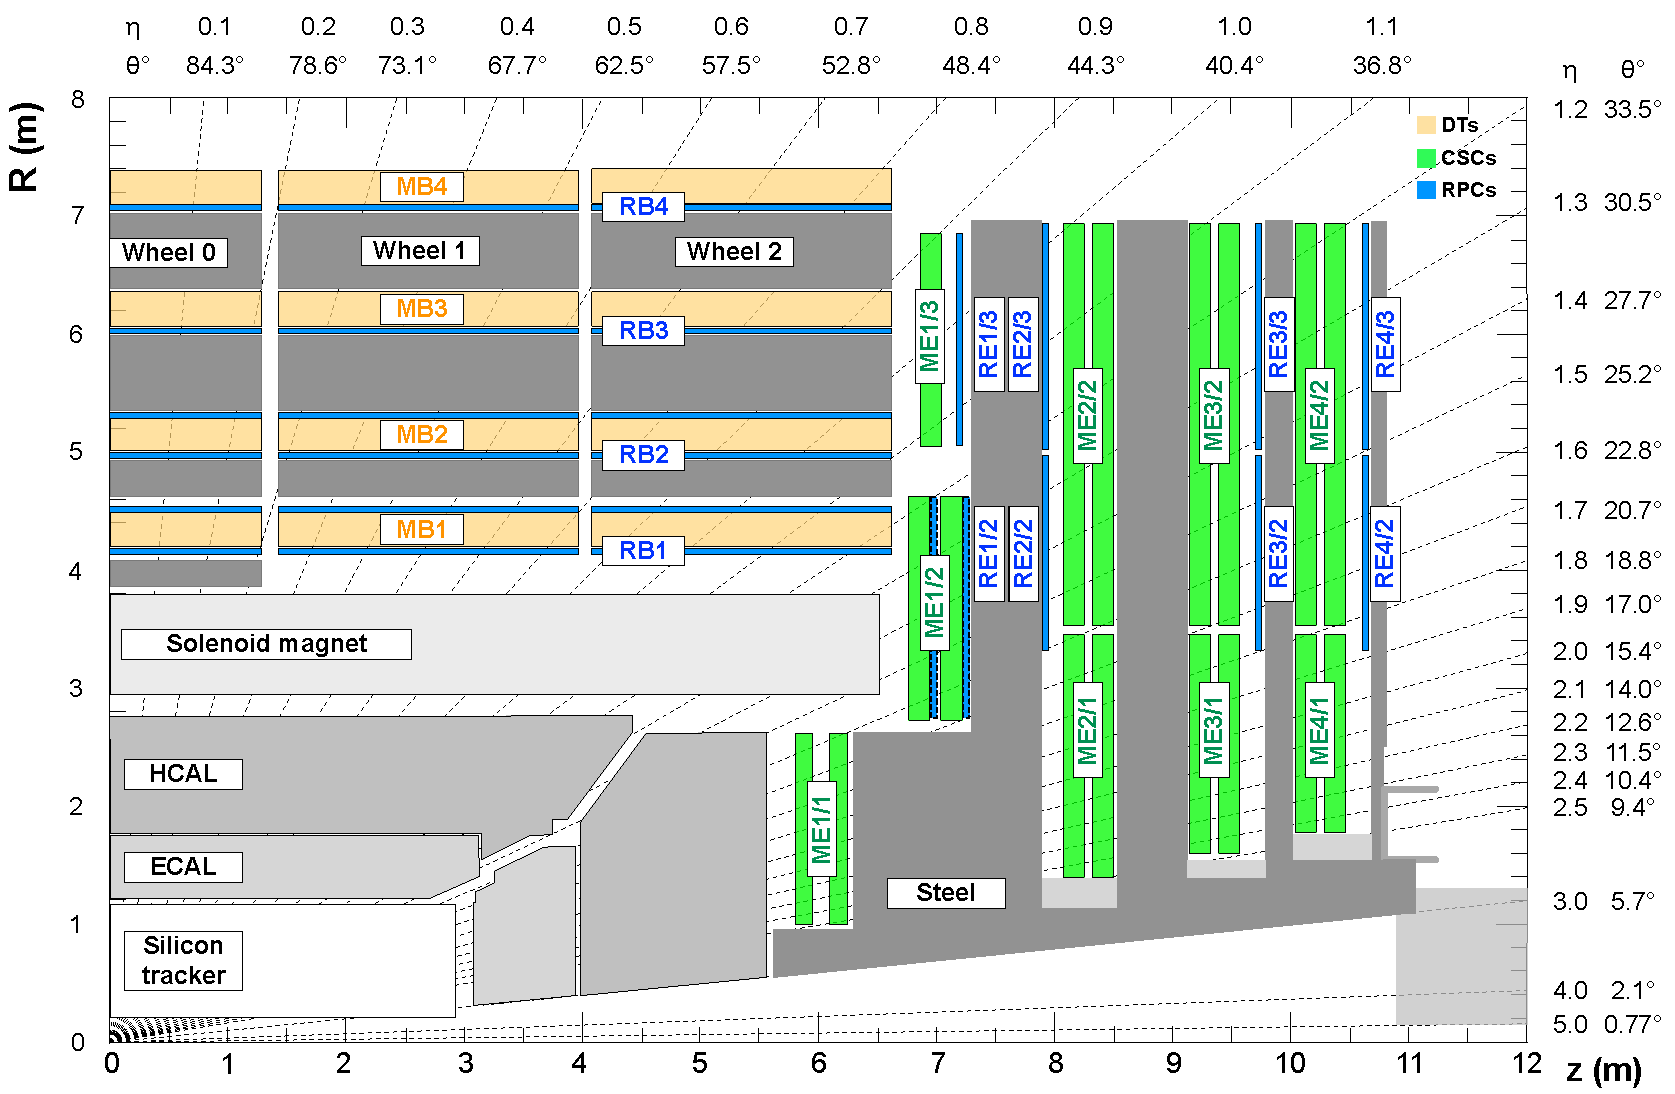
\includegraphics[width=0.97\textwidth]{figs/cms/cms_muon_quadrant_run_ii.pdf}
\caption{Layout of one quadrant in r-z of the CMS Muon Detectors in their Run II configuration (from 2015), which saw the addition of CSC and RPC disks ME 4/2 and RE 4 respectively~\cite{CMS-DP-2016-046}.}
\label{fig:muonChambers}
\end{center}
\end{figure}

The DTs operate in the barrel region across $|\eta| < 1.2$, where the magnetic field strength is low as most of the return field is contained in the iron yoke,	and each tube is $4.2\cm x 1.3\cm$ cell filled with an Ar/$CO_{2}$ mixture of 85\%/15\%.
The DT chambers are organised into four stations cylindrical of layers and for each stations, the chambers are subdivided into three ``superlayers'' (/SLs).
Each SL is comprised of four layers of DTs, where the outer SLs measure coordinates in the $r-\phi$ plane and the inner SL measures in the r-z plane (which the outermost station lacks), which provides point resolutions of $\approx 200\mum$ and a $\phi$ directional precision of $\approx 1$ mrad.

CSCs are employed in the endcaps across $0.9 < \eta < 2.4$ , where the mangetic field is non-uniform and there is a higher rate of muons than in the barrel, and are organised into four stations of concentric disks.
Initially only the inner ring of the outermost (fourth ) disk was installed, with the outer ring (ME4/2, see Fig.~\ref{fig:muonChambers}) being installed in the Long Shutdown 1 (LS1) of the LHC during 2013-2015~\cite{Battilana:2017mrm}.
Each CSC is composed of six gas gaps, with six planes anode wires running almost perpendicularly to six planes of cathode strips, and thus provides six position measurements per chamber with a precision in the $r-\phi$ plane of 75\mum for the first station and 150\mum for the other stations\cite{CMS:1997iti}.

RPCs provide coverage over $|\eta| < 1.8$, which originally only extended to $|\eta| < 1.6$, instead of the planned $|\eta| < 2.1$, for financial reasons. 
During LS1, a fourth endcap disk with RPCs was installed which extended coverage to the current coverage of $|\eta| < 1.8$\cite{Battilana:2017mrm}.
Although the RPCs have a coarser position resolution ($\approx 1\cm$) than the DTs and CPCs, have fast response times and excellent time resolution ($\approx 2\ns$).
As such, RPCs provide addition but complimentary input to trigger decisions.
A RPC is formed of two parallel resistive plates, separated by a few millimetres, with a large electric field applied across the gas filled gap.
The barrel contains six layers of RPCs, two layers in the first two stations and one in each of the outer stations, and the endcaps have 4 RPC disks each, one for each CSC station.

\subsection{Trigger and Data Acquisition Systems}\label{subsec:trigger}
At design luminosity, the LHC has a bunch crossing (BX) rate of $40\MHz$, i.e. $\approx~10^{9}$ inelastic events per second, with each proton-proton collision event having a size of $\approx 1.5MB$~\cite{Bayatian:2006nff}.
Since is is not possible to store every event or to have sufficient bandwidth to read all event off the detector, the CMS trigger system~\cite{Dasu:2000ge,Sphicas:2002gg} has to drastically reduce the data rate to the manageable level of $\approx 1\kHz$\footnote{Since initial operations, the original event storage rate of 100\Hz has been increased to 0.5 to 1\kHz}~\cite{Dasu:2000ge,phase1L1TDR}.

The vast majority of events are uninteresting from a physics perspective, with the cross sections of interesting processes being at least $\approx 10^{7}$ smaller than the total proton-proton cross section of $110.6 \pm 3.4$ mb~\cite{Antchev:2017dia}.
Therefore the CMS trigger system is designed to, within the constraint of the design readout and storage capacity, reject these background events and selecting events in a manner that allows all possible new physics signatures to be detected whilst keeping acceptance thresholds sufficiently as low as reasonably possible.
The CMS trigger system is comprised of two stages, The Level-1 (L1) Trigger and the High Level Trigger (HLT), as it not feasible to reduce the data rate in a single processing stage without compromising on physics performance.

\subsubsection{L-1 Trigger}\label{paragraph:L1}
The Level-1 Trigger reduces the raw $40\MHz$ rate to $\approx100\kHz$ and consists of FPGAs (Field Programmable Gate Arrays) and ASICs (Application Specific Integrated Circuits), which have to identify hard scattering physics signals at a high efficiency with acceptance thresholds as low as possible, within constraint of the system having to analyse every bunch crossing (BX).
The strict time limitations on how long it takes for the data can be collected and read out, precludes both the reading out of events in full and of the use of iterative reconstruction algorithms.
As the selection cannot be done before the subsequent BX, given the above constraints, the L1 Trigger uses a pipelined approach which provides a total system latency of $\approx$ 3.8\mus, during which the detector data is buffered (the Tracker and ES buffers being the limiting factor of the system latency) prior to either being read out or discarded.
The L1 acceptance decision is based on whether ``trigger primitives'' formed from promptly available data from the ECAL, HCAL or muon detectors above the pre-determined \pT or \ET thresholds.
Tracking information is not used in the L1 Trigger as its inclusion was determined to be unnecessary for nominal LHC conditions, and consequently, it has not been designed to be read out for every event.

Given that following LS1 it was planned that both the instantaneous luminosity and centre-of-mass energy of the LHC were to increase, the Phase-I Trigger Upgrade~\cite{Tapper:2013yva} was undertaken in order to prevent the physics program being compromised from a substantial increase in the trigger thresholds that would be required to maintain the 100\kHz L1 trigger limit.	
This requirement has been met by a flexible design based on a large FPGAs on a small number of general-purpose boards which are able to perform more sophisticated identification and reconstruction algorithms over the entire detector without regional boundaries.
The upgraded electronics of the Phase-I Trigger were installed during LS1 and ran using the legacy trigger system during 2015 with the new trigger system (Fig.~\ref{fig:trigger}) running in parallel for validation prior to commissioning and usage during 2016~\cite{Zabi:2017lya}.
%%% Old text
%Initially both the calorimeter and muon triggers search over a small local area for the signature of an interesting event, forwarding these onto the regional triggers which sorts the candidates in order of importance, before the global calorimeter and muon triggers determine the highest ranked objects across the entire experiment. 
%These are sent to the Global Trigger, which either rejects an event or accepts it for further evaluation by the second step, the High-Level-Trigger (HLT), a software system (see Fig.~\ref{fig:trigger} for a more detailed breakdown). 
%Events accepted by the HLT are then transferred to mass storage for offline storage and analysis\cite{oldcms}. 
%In light of this, the current approach of having large amounts of data over small regions being brought to fewer boards so that objects of interest can be considered, has to discard data at each stage a larger region is considered . 
%While this approach creates candidates within these constraints, by definition only the candidates from this coarser data set can be considered. 
%Any candidates in the discarded data are lost\cite{oldcms}.
%%%

\begin{figure}[htbp]
\begin{center}
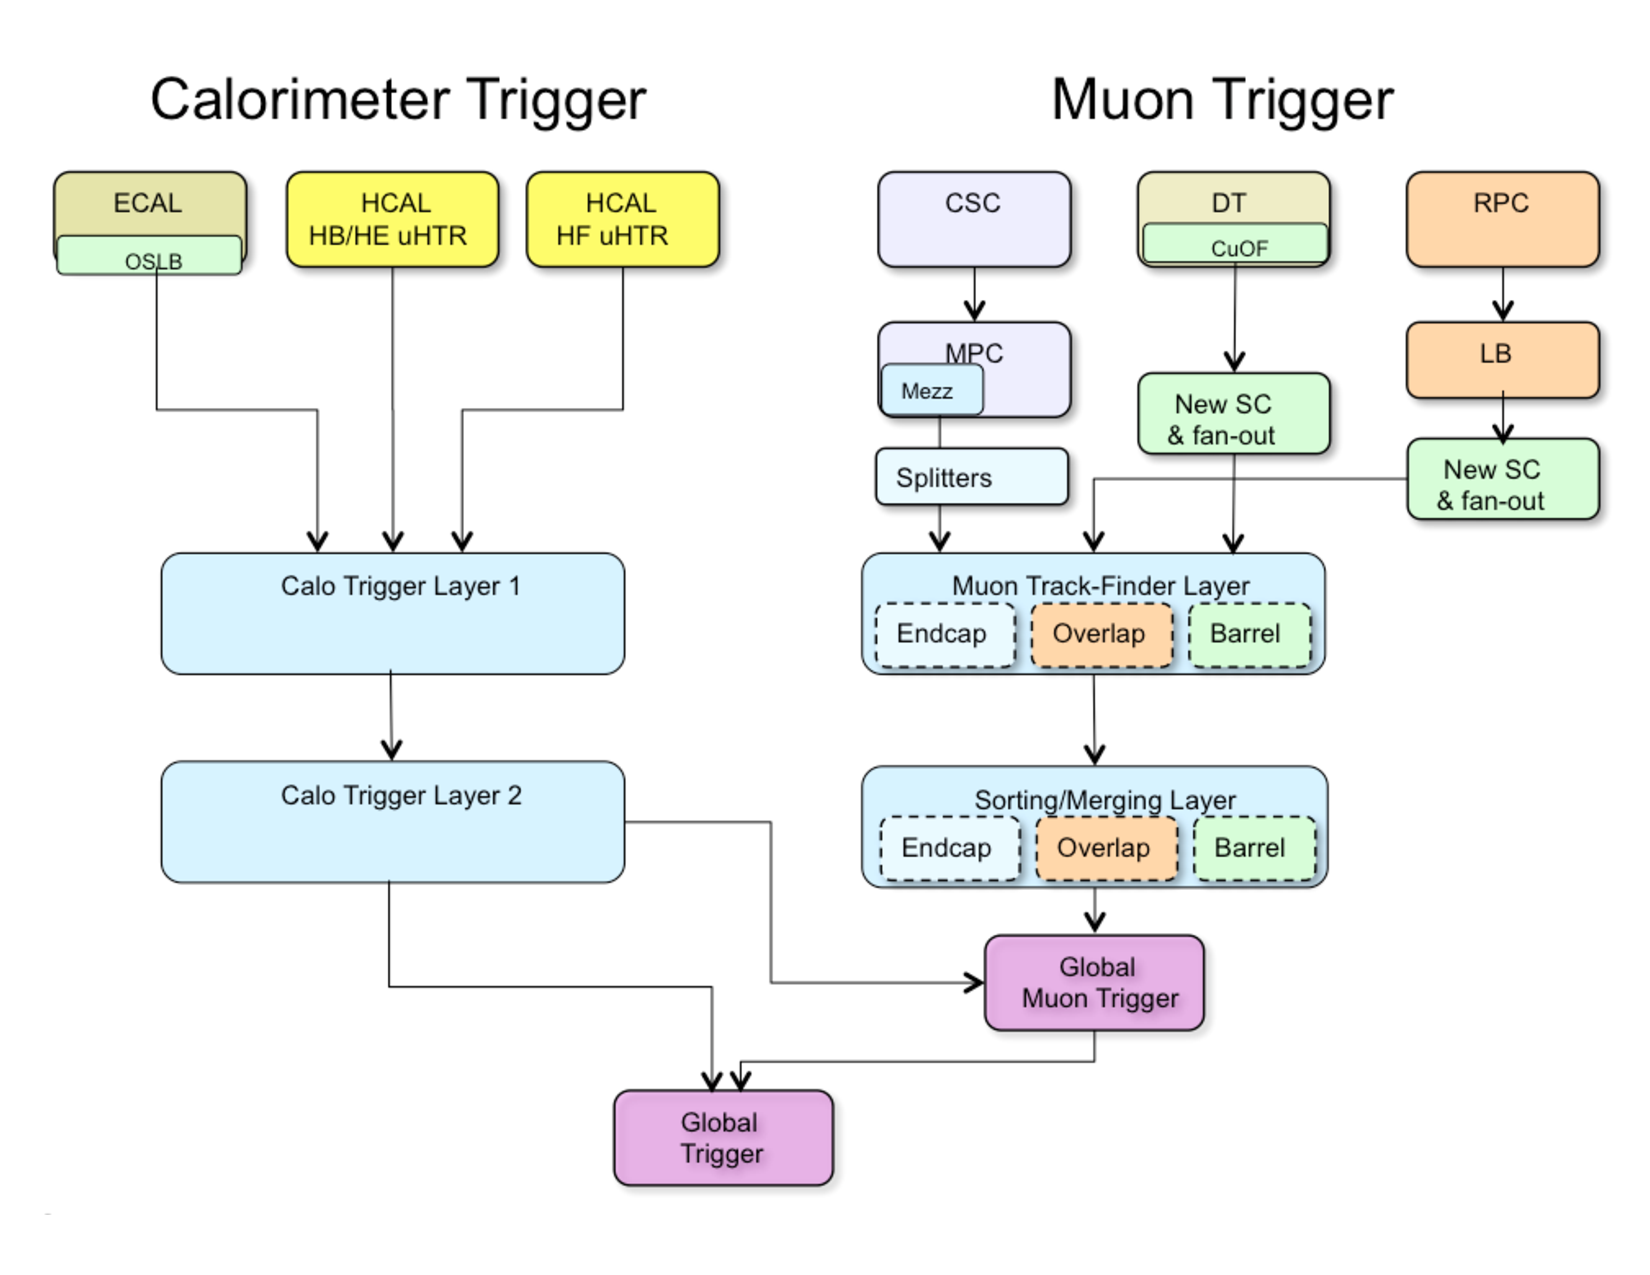
\includegraphics[width=0.97\textwidth]{figs/cms/TrigUpgradeBlockDiagram.pdf}
\caption{Current (Phase-I) Level-1 Trigger Architecture~\cite{Tapper:2013yva}.}
\label{fig:trigger}
\end{center}
\end{figure}

\subsubsection{High Level Trigger and Data Acquisiation}\label{paragraph:HLT}
Upon receipt of a L-1 trigger, the Data Acquisition (DAQ) system (Fig.~\ref{fig:DAQ}) reads out the buffered data from the detector Front-End Drivers, buffers it in the Readout Systems until the Builder Network (controlled by the Event Manager) can transfers data to the Filter Systems where the event fragments are collated into a complete event and processed through the HLT algorithms~\cite{Sphicas:2002gg}. 

\begin{figure}[htbp]
\begin{center}
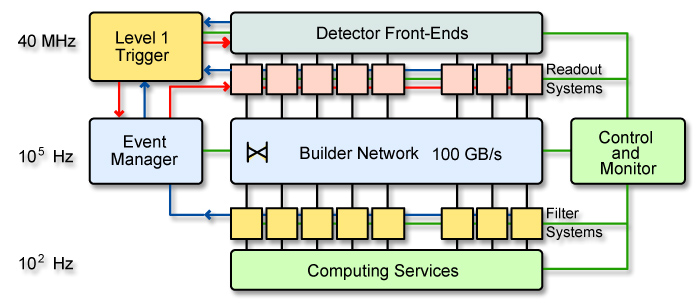
\includegraphics[width=0.97\textwidth]{figs/cms/CMS_DAQ.jpg}
\caption{Overview of the CMS Data Acquisition system architecture~\cite{Sphicas:2002gg}.}
\label{fig:DAQ}
\end{center}
\end{figure}

The HLT reduces the L1 rate of $\approx 100\kHz$ to the output rate of $\approx 1\kHz$.
In contrast to the L1 trigger, the HLT algorithms are performed by commercially available processors by the CMS Software (\CMSSW), which allows for great flexibility of alogirthms and the use of the full detector readout (including the Tracker and ES) to reconstruct the event and select events.
Given that the the time limitations on the HLT are not as strict as the L1 Trigger, with events requiring an average of $\approx 40\ms$, more sophisticated reconstruction and selection algorithms are used.
This however, does not mean that the full event is reconstructed, as such a task is too CPU intensive to be done online within the latency constraints.
The output from the Filter System is collected by the Computing Services and forwarded to the offline Tier-0 computing centre for offline processing and reconstruction and to the detector's online monitoring systems.
